\documentclass[final]{beamer}

% ====================
% Packages
% ====================

\usepackage[T1]{fontenc}
\usepackage{lmodern}
\usepackage[size=custom,width=118.9,height=84.09,scale=1.0,orientation=landscape]{beamerposter}
\usetheme{gemini}
\usecolortheme{cam}
\usepackage{graphicx}
\usepackage{booktabs}
\usepackage[numbers]{natbib}
\usepackage{tikz}
\usepackage{pgfplots}
\pgfplotsset{compat=1.14}
\usepackage{anyfontsize}

% ====================
% Lengths
% ====================

% If you have N columns, choose \sepwidth and \col           width such that
% (N+1)*\sepwidth + N*\colwidth = \paperwidth
\newlength{\sepwidth}
\newlength{\colwidth}
\setlength{\sepwidth}{0.025\paperwidth}
\setlength{\colwidth}{0.3\paperwidth}

\newcommand{\separatorcolumn}{\begin{column}{\sepwidth}\end{column}}

% ====================
% Title
% ====================

\title{LHCbFinder: Semantic Search and Knowledge Discovery Framework}

\author{Mohamed Elashri \and Conor Henderson \and Michael David Sokoloff}

\institute[shortinst]{University of Cincinnati \& LHCb Collaboration}

% ====================
% Footer
% ====================

\footercontent{
  7th Inter-Experimental LHC Machine Learning Workshop - 2025 \hfill
  \href{mailto:mohamed.elashri@cern.ch}{mohamed.elashri@cern.ch}}

% ====================
% Logo
% ====================

% use this to include logos on the left and/or right side of the header:
\logoright{
\includegraphics[height=6cm]{lhcb-logo.jpg}}
\logoleft{
\includegraphics[height=6cm]{uc-logo.jpg}}

% ====================
% Body
% ====================

\begin{document}

\begin{frame}[t]
\begin{columns}[t]
\separatorcolumn

\begin{column}{\colwidth}

  \begin{block}{Vision and Motivation}
    \textbf{Current Knowledge Management Challenges at LHCb:}
    \begin{itemize}
      \item \textbf{Fragmented knowledge} across multiple platforms (TWiki, Indico, arXiv, internal notes)
      \item \textbf{Valuable institutional knowledge} often undocumented or difficult to discover
      \item \textbf{Steep learning curve} for newcomers joining the collaboration
    \end{itemize}

    \textbf{LHCbFinder Solution:}
    \begin{itemize}
      \item Centralize scattered documentation in a semantic framework
      \item Enable intuitive natural language search across all resources
      \item Preserve and share institutional knowledge
      \item Reduce entry barriers for new members
    \end{itemize}
  \end{block}

  \begin{block}{Semantic Search Foundation}
    
    LHCbFinder employs a powerful semantic search pipeline that forms the foundation of our knowledge platform:
    
    \begin{figure}
      \centering
      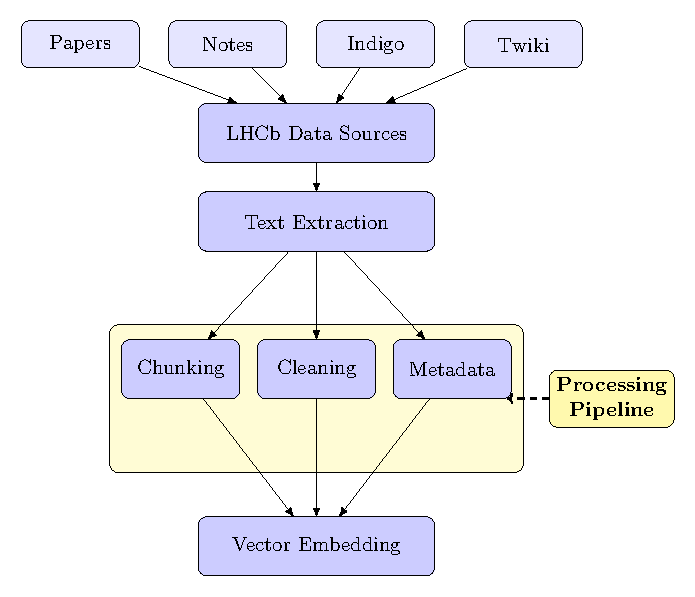
\includegraphics[width=0.85\textwidth]{figure1-text-processing.pdf}
      \caption{Text processing pipeline for creating vector embeddings}
    \end{figure}

    \textbf{Strategic Implementation:}
    \begin{itemize}
      \item \textbf{Phase 1:} Abstracts for rapid validation
      \item \textbf{Phase 2:} Full paper introductions for deeper context
      \item \textbf{Phase 3:} Comprehensive scaling to all document types
    \end{itemize}

  \end{block}

  \begin{alertblock}{Key Features}
    
    Our semantic search system offers significant advantages over traditional keyword search:
    
    \begin{itemize}
      \item Understands meaning and context rather than just matching keywords
      \item Finds conceptually related documents using vector similarity
      \item Supports natural language queries for intuitive discovery
    \end{itemize}
    
  \end{alertblock}

\end{column}

\separatorcolumn

\begin{column}{\colwidth}

  \begin{block}{Understanding Embeddings and Vector Search}

    The heart of LHCbFinder is our embedding system that converts scientific text into semantic vectors:

    \begin{figure}
      \centering
      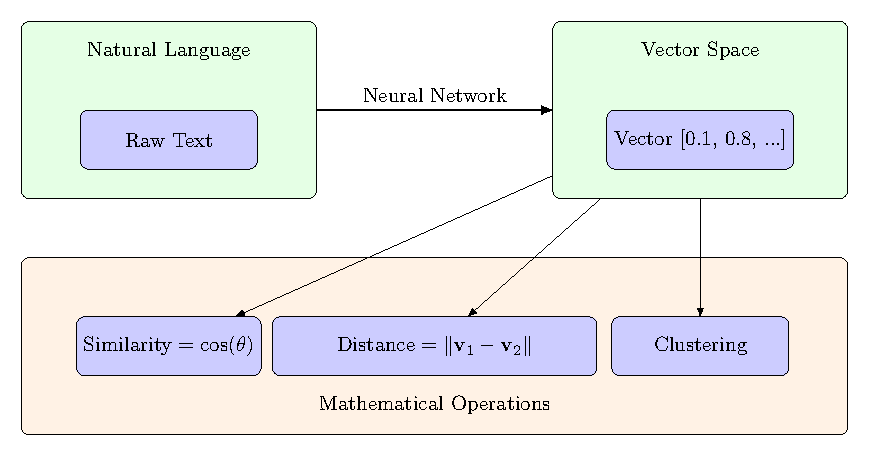
\includegraphics[width=0.95\textwidth]{figure2-embeddings.pdf}
      \caption{Converting text to vectors for semantic search}
    \end{figure}
    
    \textbf{Embedding Model:} BAAI/bge-large-en-v1.5
    \begin{itemize}
      \item 1024-dimensional vector embeddings
      \item Optimized for scientific literature
      \item Excellent technical term handling
    \end{itemize}
    
    \textbf{Vector Database:}
    \begin{itemize}
      \item Efficient similarity search with ChromaDB (local) and Pinecone (cloud)
      \item Scales to millions of vectors
      \item Supports hybrid deployment for flexibility
    \end{itemize}
    
  \end{block}

  \begin{block}{RAG: Retrieval-Augmented Generation Framework}
    
    The next phase of LHCbFinder integrates LLMs with our vector knowledge base:
    
    \begin{figure}
      \centering
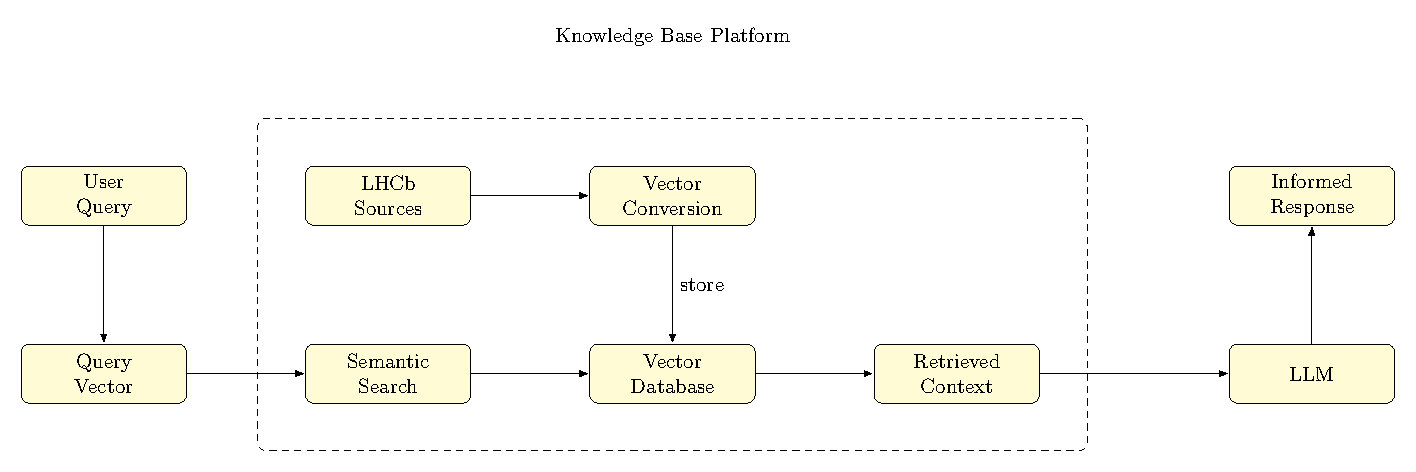
\includegraphics[scale=1.4]{figure3-rag-architecture.pdf}
      \caption{Retrieval-Augmented Generation architecture}
    \end{figure}
    
  \end{block}

\vspace{5cm}
  \begin{exampleblock}{Live Demo and Current Status}
    
    \textbf{lhcbfinder.net} offers semantic search across LHCb papers with natural language queries. Try searches like \textit{"CP violation in B decays"} or \textit{"Machine learning for tracking"} to explore related papers ranked by semantic similarity.
    
    
  \end{exampleblock}

\end{column}

\separatorcolumn

\begin{column}{\colwidth}

  \begin{block}{Development Roadmap}
    
    % Increased row spacing and font size
    \begin{tabular}{p{0.25\textwidth}|p{0.65\textwidth}}
      \multicolumn{2}{c}{\Large \textbf{Three-Phase Strategy}} \\[0.4cm]
      
      \large \textbf{Phase 1: Foundation} \newline
      \large \textit{Current} &
      \large Full semantic search for LHCb papers. Optimized embeddings and refined user experience. \\[1.2cm]
      
      \large \textbf{Phase 2: Integration} \newline
      \large \textit{Next} &
      \large Developing document scraping/knowledge grabbing pipeline for diverse LHCb resources and integrating with LLM models. \\[1.2cm]
      
      \large \textbf{Phase 3: Expansion} \newline
      \large \textit{Future} &
      \large Framework-agnostic development to extend beyond LHCb, enabling knowledge discovery across different HEP experiments. \\[0.8cm]
    \end{tabular}
    
    \vspace{0.5cm}
    
    \large \textbf{Current Priorities:} Content acquisition, framework modularization, and LLM integration.
    
  \end{block}

  \begin{block}{Technical Implementation}
    
    \textbf{System Architecture:}
    
    \begin{figure}
      \centering
      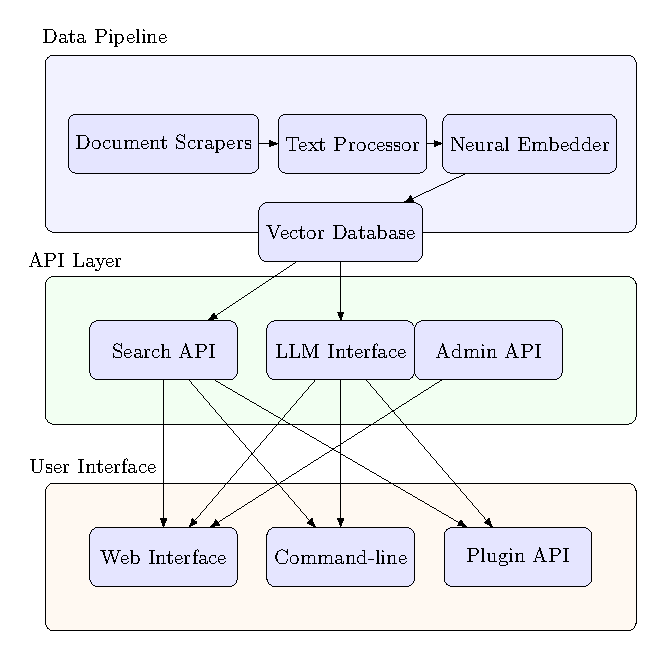
\includegraphics[width=0.85\textwidth]{figure4-system-architecture.pdf}
      \caption{LHCbFinder system architecture}
    \end{figure}
    
  \end{block}

  \begin{alertblock}{Future Research Directions}
    
    \textbf{LHC-Specific Embedding Models:}
    Training specialized vector embeddings on physics domain terminology to improve semantic understanding of technical concepts in HEP documentation.
    
    \textbf{LLM Integration Framework:}
    Evaluating various open-source LLMs for compatibility with scientific knowledge retrieval, including benchmarking domain-specific response quality.
    
    \textbf{Experiment-Agnostic Architecture:}
    Developing a modular design to extend beyond LHCb, enabling knowledge discovery across all LHC experiments with minimal adaptation.
    
  \end{alertblock}


\end{column}

\separatorcolumn
\end{columns}
\end{frame}

\end{document}